% ##################################################################################################################
\chapter{The SmartBay Project: Connected Mobility in San Francisco Bay Area}
\label{ch:sanfrancisco}
\hfill \textbf{Author:} Alexei Pozdnoukhov, Andrew Campbell, Sidney Feygin, Mogeng Yin, Sudatta Mohanty

\editdone{This text has undergone the professional edit. Please no grammatical changes anymore! They are most-probably wrong.}

% ##################################################################################################################
\section{Introduction}
Novel mobility-as-a-service paradigm, enabled by \gls{ict} and mobile computing, is changing the transportation landscape faster than traditional data sources, such as travel surveys, are able to reflect. The development of on-demand transportation, the rising popularity of car- and ride-sharing services and the growing tendencies towards multi-modality pose new challenges for supply side modeling. This is particularly true in the San Francisco Bay Area (California, USA) as the influx of people and businesses to the city, volatility of job markets, evolving demographics and internal migration further increase the variability of mobility patterns evolution. It is more important than ever to be able to measure, realistically model and forecast travel demand in near real-time. The baseline scenario of the SmartBay project spans the nine counties in the area and is designed to extend the state-of-the-art in activity-based simulations in two respects. First, the SmartBay's demand model is based on the anonymized cellular network infrastructure data stream. Second, agents' population is connected to a social network and their scoring functions are tailored to study the implications social influence exerts, particularly in mode and secondary destinations locations choice. 

 %------------
\createfigure%
{The geographical extent of the SmartBay simulation (left) and a close-up view on the \gls{multimodal} network spanning San Francisco-Oakland area (right)}%
{The geographical extent of the SmartBay simulation (left) and a close-up view on the \gls{multimodal} network spanning San Francisco-Oakland area (right)}%
{\label{fig:sf1}}%
{%
 \createsubfigure%
 {}
 {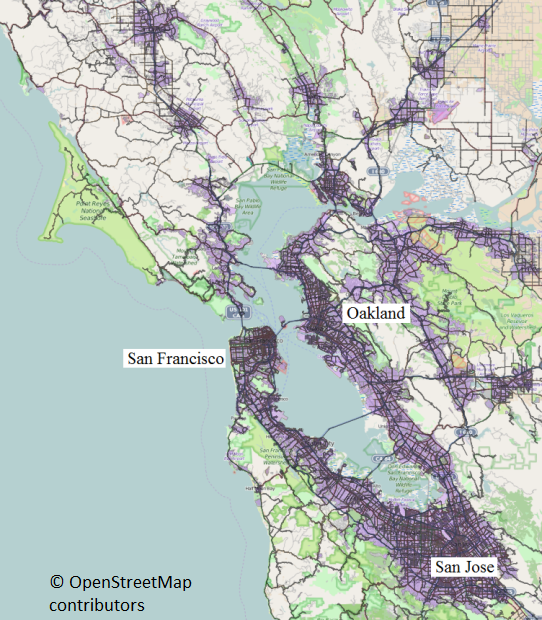
\includegraphics[width=0.44\textwidth, angle=0]{./scenarios/figures/sf_fig1_left.png}}
 {\label{fig:sf_fig1_left}}
\createsubfigure%
 {}
 {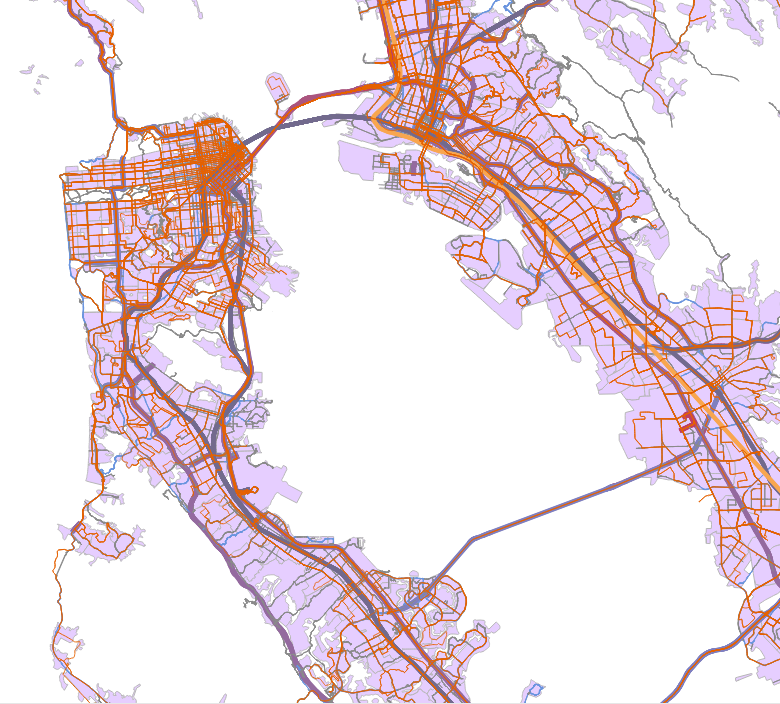
\includegraphics[width=0.54\textwidth, angle=0]{./scenarios/figures/sf_fig1_right.png}}
 {\label{fig:sf_fig1_right}}
}%
{}
 %------------
% ##################################################################################################################
\section{The Study Area and Networks}
The baseline SmartBay simulation implements a typical working day scenario within the nine San Francisco Bay area counties. As of 2015, total area population is 7.5\,M people, with an estimated 3.4\,M commuters, of whom 350\,K use public transport as their only commute mode. Driving is the major mode for home to work trips, with 75\,\% of trips made by a driver alone. While average commute duration is estimated to be 28\,minutes, severe congestion at peak hours is widespread. The road network used in the scenario consists of a total of 96\,000\,links, with a mix of freeways, state routes, all major arterial and countryside roads. Road network geometries were extracted from the \gls{osm} data: then verified and augmented with the speed limits, capacities and number of lanes. The network was extended with all major public transit lines available through \gls{gtfs}, provided by the respective agencies. There are 9\,major bus agencies, several minor bus line operators, a light rail system, and commuter trains. The major rapid rail carrier is a Bay Area Rapid Transit system that serves 400\,K daily trips over four inter-connected lines. \gls{gtfs} includes schedules and capacities of transit vehicles.

% ##################################################################################################################
\section{Population and Demand Generation}
There are 1454\,\glspl{taz} in the area developed by the \gls{mtc}, used as origin and destination units of a demand model developed and supported by the \gls{mtc}, as well as for population and workplace projections made on a regular basis for different time horizons. The \gls{mtc} model adopts the activity-based approach, with a tour-trip hierarchy of mandatory (home, work, school trips) and secondary trips, with the respective mode choices, composition of tours and departure times governed by a rich set of discrete choice models calibrated from recent California Household Travel Survey data (CHTS, 2010-2012) and inherited from other California agencies' relevant studies. 

SmartBay scenarios use the anonymized cell phone data logs to adjust \gls{mtc} demand models. Cell phone data are routinely collected and managed by AT\&T Inc., the second largest nationwide telecom operator in the United States with 120\,M users nationwide (which translates to a sample size of more than 1\,M commuters in the SF Bay Area). Data used for mobility modeling originates from anonymized \glspl{cdr}, recorded at the spatial resolution of the deployed cell phone towers (or antennas) and is usually available with a time latency of several minutes. Historical \glspl{cdr} analysis allows detection of important places for each user based on  frequency of calls, texts or data packets sent through a given cell tower \citep[][]{IsaacmanEtAl_LNCS_2011, BeckerEtAl_CACM_2013}. This approach is most robust in identifying primary locations of frequent and recurrent visits, such as home, work or school. The data is stored and processed internally at secure AT\&T servers. A rescaling procedure, based on area-to-point pycnophylactic interpolation \citep[][]{KaiserEtAl_PMC_2013} and a variant of iterative proportional fitting was used to project aggregates from cell tower level to areal units defined by the \glspl{taz}. Population census data were used to estimate correction coefficients and adjust cell phone user counts for the total population. This adjustment resulted in an up-to-date and more accurate representation of mandatory trip \gls{od} flows related. When compared with the \gls{mtc} demand models, notable discrepancies detected include new urban developments, as well as major shifts in employment re-distribution due to the fast IT sector evolution in Silicon Valley.

% ##################################################################################################################
\section{Work Commute Model Evaluation}
\gls{matsim} instance was deployed on AT\&T servers to simulate the home-to-work commute scenario for a typical weekday. Scenario runs with 15\,\% to 30\,\% commuting population sample were evaluated (550\,K to 1.1\,M agents). Driving and public transit were set as the only modes; mode share at the beginning of the mode re-planning in \gls{matsim} was set according to \gls{mtc} findings from CHTS. Resulting link volumes were validated based on hourly traffic counts collected by California Department of \gls{pems} inductive loop detectors, deployed on all major freeways. Sample count histograms are presented in Figure~\ref{fig:sf_fig2}. The model met the Federal Highway Authorities accuracy specifications.

 %------------
\createfigure%
{A sample of the simulated vehicles and the examples of the observed (light/orange) and simulated (dark/blue) counts at two particular validation locations. Secondary trips, mainly occurring at midday, were not included in this scenario}%
{A sample of the simulated vehicles and the examples of the observed (light/orange) and simulated (dark/blue) counts at two particular validation locations. Secondary trips, mainly occurring at midday, were not included in this scenario}%
{\label{fig:sf_fig2}}%
{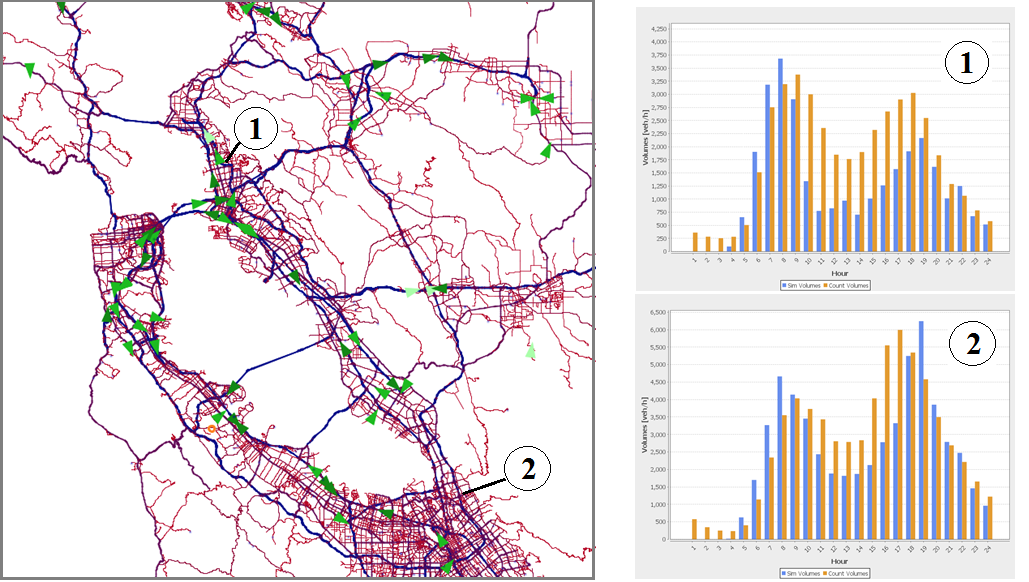
\includegraphics[width=0.99\textwidth, angle=0]{./scenarios/figures/sf_fig2.png}}%
{}
 %------------

% ##################################################################################################################
\section{Extensions and Work in Progress}
Main extensions developed in the SmartBay project are related to simulating a population explicitly connected to a social network; current work is directed toward two domains. First, an extension of location choice is approached with machine learning tools that model social influences in destination choices for secondary activities and the second extension introduces social connections to scoring functions and aims to capture peer pressure effects in mode choices.

% =============================================================================
\paragraph{Social Influence in Destination Choice}
There is evidence that population social network geography in an area is a strong predictor of destination choice for secondary trips. This is valid both for trips directly related to social activities, as well as when destination choice was conditioned by recommendations received from peers in the past. As such, this provides a way to use machine learning-based approaches for predicting destination choice from historical data and social ties. This approach requires building a  social connections model for the virtual agent population, \ie defining a weighted graph with edges $P_{ij}$ for each pair of agents $i$ and $j$. Our preliminary work is based on the model proposed in \citet[][]{McGrathPozdnukhov_UrbComp_2014} and is applied at the home level \glspl{taz}, instead of an individual. This approach requires a seed network to be derived from the cell phone \glspl{cdr}, with the weights $P_{ij}$ emphasizing recurrent reciprocal calls, as evidence of a social tie between $i$ and $j$. The seed network is then removed from the model, resulting in a connected virtual population with similar network statistics that replicates the geographical community's real social network structure in the area. 

SmartBay currently adopts the \gls{mtc}  secondary activities classification that includes eight categories for non-mandatory trips. There are 120\,K venues derived from the \lstinline|Factual.com| \gls{api}, introduced to the simulation as destinations for secondary trips. Hierarchical spatial clustering was applied to the venues set to reduce the number of venues to 1\,200. This approach is justified both by the need to reduce computational expenses in the re-planning stage, as well as evidence of spatial hierarchies in human spatial cognition and decision making. A spatial choice model for the secondary home- and work-based trips is calibrated from the \glspl{cdr}, using the \citet[][]{McArdleEtAl_ACMTIS_2014} approach. A key  parameter set in this model is the attractiveness of agent venues, which is assumed to be proportional to the number of peers who also visit the venue. A thorough experimental validation of the full-scale scenario, with secondary trips, is computationally expensive and is ongoing.

% =============================================================================
\paragraph{Social Influence in Mode Choice} 
The following extension to the conventional Charypar-Nagel scoring function is considered:
\begin{equation*}
U_i=U_i^{CN}-\gamma\sum_{j=1}^N P_{ij}\left\Vert a_i - a_i^0 \right\Vert +\theta \sum_{j=1}^N P_{ij} \left\Vert a_i - a_j \right\Vert
\end{equation*}

Here, an agent specification is extended with an attribute vector $a_i$, describing an agent's profile as it relates to membership in a particular group (such as drivers or transit users). We define attribute components as continuous within $\left[0, 1\right]$ interval, corresponding to an agent's tendency to drive or take transit as his/her primary commute mode. This attribute value is also used to define the probability of the current plan's primary mode choice to be selected for mutation in the evolutionary optimization re-planning step. $U_i^{CN}$ represents the Charypar-Nagel score of the daily plan, augmented with two terms. The first term describes peer pressure effect toward a pre-specified ``socially-responsible'' choice $a_i^o$. The second term describes an agent's tendency to behave similarly to his/her immediate peers in regard to choice attributes. As these two effects appear only with evidence of a social tie, both terms include a summation over the agent peers, with connection strength $P_{ij}$ defined as described in the previous subsection. The resulting mode choice sensitivity to parameter values $\gamma$ and $\theta$ is determined through currently ongoing computational experimentation.

% ##################################################################################################################
\section{Conclusions and Acknowledgments}
An increasing pace of urbanization severely tests city infrastructure systems. The transportation field is responding to these global challenges by evolving at an ever-increasing pace. More flexible and powerful tools are required to support decision making in planning, operations, and policy regulation applied to emerging mobility technologies. SmartBay project has developed a \gls{matsim}-based platform capable of ingesting demand models based on big data and extending the utility functions specifications to study social influence on mobility behaviors. It also incorporates semi-parametric machine learning models applied to destination location choice predictions for socially-related secondary trips. With encouraging results obtained in baseline scenario simulations, these advanced developments are currently ongoing. 

The authors acknowledge the contributions from our collaborators at AT\&T Research: Dr.~J.-F.~Paiement, Dr.~J.~Pang, Dr.~A.~Skudlark, Dr.~C.~Volinsky. Funding support from State of California Department of Transportation (CalTrans) through UCCONNECT faculty research grant program, agreement 65A0529, is also acknowledged.

% ##################################################################################################################     




